\documentclass[12pt, twoside]{article}
\usepackage{jmlda}
\newcommand{\hdir}{.}

\newtheorem{theorem}{Теорема}
\newtheorem{lemma}[theorem]{Лемма}
\newtheorem{definition}{Определение}


\begin{document}

\title
    {Обучение с экспертами для выборки со многими доменами} % Название
\author
    {Н.\,А.~Линдеманн, А.\,В.~Грабовой} % основной список авторов, выводимый в оглавление
\email
    {lindemann.na@phystech.edu; andriy.graboviy@mail.ru}
%\thanks
%    {Работа выполнена при
%     %частичной
%     финансовой поддержке РФФИ, проекты \No\ \No 00-00-00000 и 00-00-00001.}
%\organization
%    {$^1$Организация, адрес; $^2$Организация, адрес}
\abstract
    {Рассматривается задача аппроксимации multi-domain выборки единой мультимоделью -- смесью экспертов. Каждый домен аппроксимируется локальной моделью. В работе рассматривается двухэтапная задача оптимизации на основе ЕМ-алгоритма. В качестве данных используется выборка отзывов сайта Amazon для разных типов товара, которая содержит в себе несколько доменов. В качестве локальной модели используется линейная модель, а в качестве признакового описания отзывов используются tf-idf вектора внутри каждого домена.

	
\bigskip
\noindent
\textbf{Ключевые слова}: \emph {Смесь экспертов, локальная модель, обучение с экспертом, классификация текстов.}

}

%данные поля заполняются редакцией журнала
%\doi{10.21469/22233792}
%\receivedRus{01.01.2017}
%\receivedEng{January 01, 2017}

\maketitle
\linenumbers

\section{Введение}
На текущий момент в машинном обучении появляется все больше задач связанных с данными, которые взяты с разных источников. Часто появляются выборки, которые состоят из большого количества доменов. Под \textit{доменом} понимается подмножество объектов выборки, которые обладают некоторыми одинаковыми признаками. На текущий момент не существует полного теоретического обоснования построения смесей локальных моделей для аппроксимации такого рода выборок. 

В работе рассматривается задача аппроксимации multi-domain выборки единой мультимоделью -- смесью экспертов, и предлагается алгоритм бинарной классификации текстов, использующий дополнительную информацию о доменах. Использование этой информации позволяет использовать более простые и интерпретируемые модели.

Метод решения задачи состоит в построении мультимодели, являющейся смесью локальных моделей. Каждый домен аппроксимируется локальной линейной моделью, смесь которых является итоговым алгоритмом классификации. Задача обучения модели сводится к двухэтапной задаче оптимизации на основе ЕМ-алгоритма. Схема работы алгоритма представлена на рис.~\ref{example:1}.

\begin{figure}[H]\center
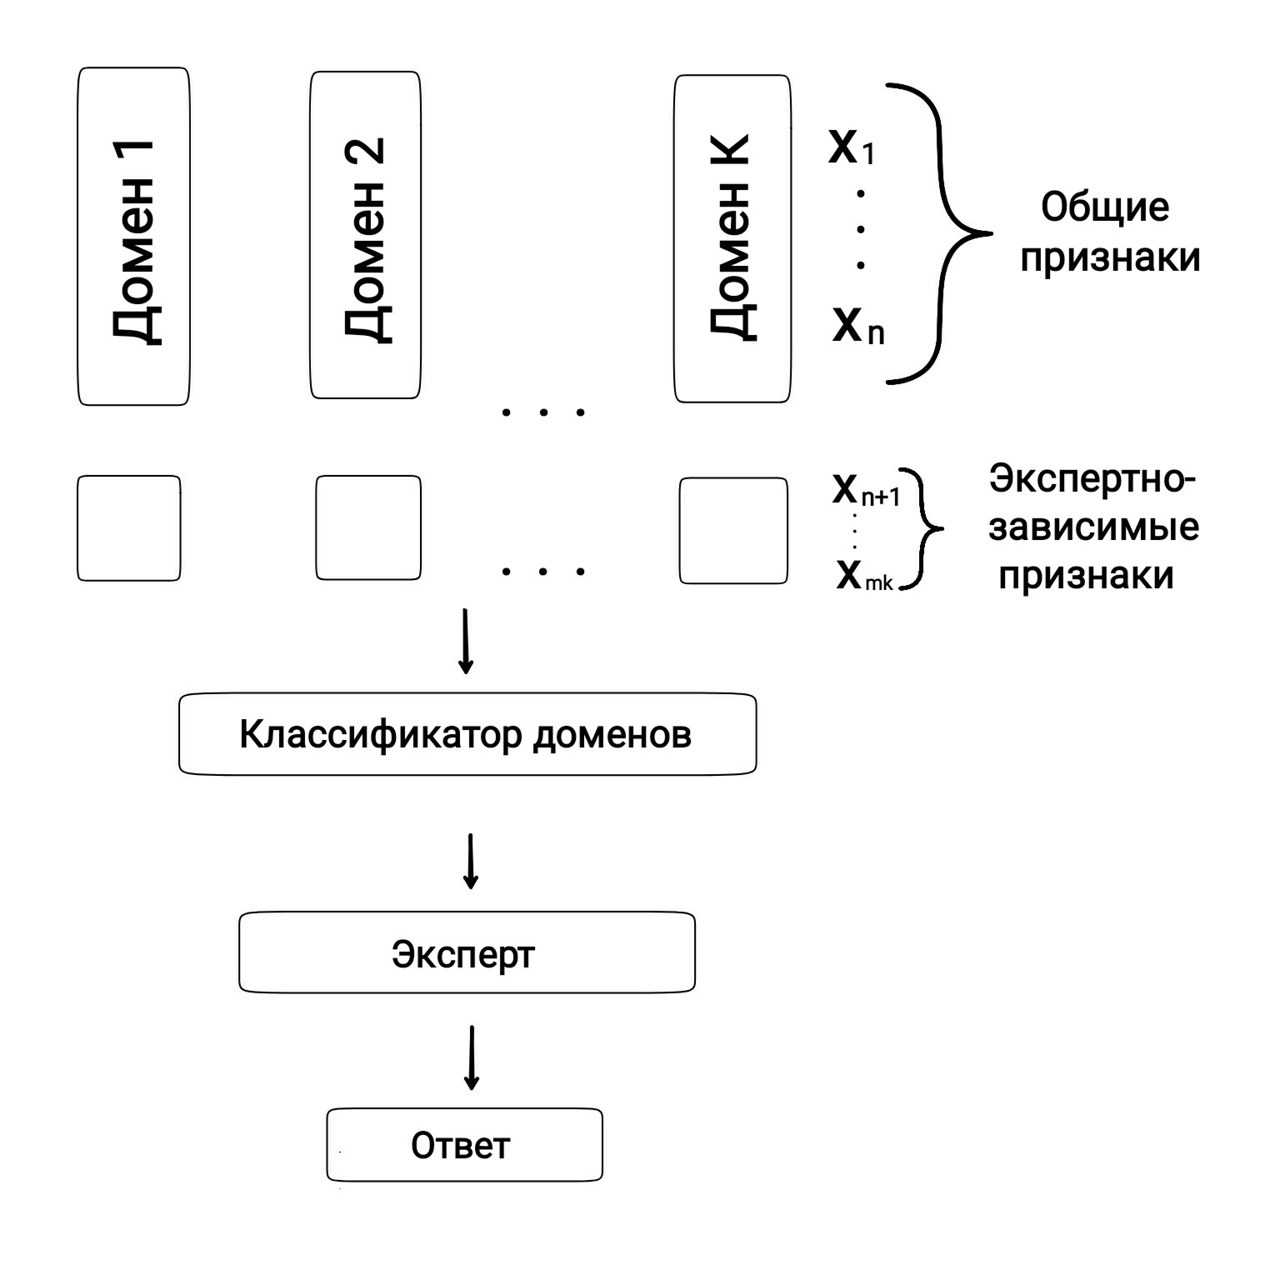
\includegraphics[width=0.5\textwidth]{Schem_1.jpg}
\caption{Схема работы мультимодели.}
\label{example:1}
\end{figure}

В качестве данных используется выборка отзывов сайта Amazon для разных типов товара, которая содержит в себе несколько доменов. Каждый объект имеет экспертно-зависимое описание, которое определяется его пренадлежностью к тому или иному домену. В качестве признакового описания отзывов используется tf-idf вектора внутри каждого домена. 


\section{Постановка задачи}
\subsection{Постановка задачи обучнения одного эксперта}
Задача бинарной классификации является задачей апроксимации целевой функции
\[
\label{eq:st:1.1}
\begin{aligned}
\mathbf{f}: \mathbb{R}^n \to \{-1, +1\},
\end{aligned}
\]
где $\mathbb{R}^n$ -- пространство признакового описания объектов, а $\{-1, +1\}$ -- метка класса объекта. Задачей локальной модели является апроксимация функции $\mathbf{f}$ на некотором домене. На основе общих признаков $(x_1, \ldots, x_n)$ эксперт генерирует экспертно-зависимые признаки $(x_{n+1}, \ldots, x_{m_k})$, количество которых зависит от конкретного домена, и с помощью признаков $(x_1, \ldots, x_nб x_{n+1}, \ldots, x_{m_k})$ локальная модель делает предсказание о принадлежности объекта к одному из двух классов.

В качестве локальной модели будем использовать логистическую регрессию, которая будет предсказывать вероятность того, что объект с признаковым описанием $\vec{x_i}$ принадлежит классу $y_i$:
\[p\left(y = y_i \mid \vec{x_i}, \mathbf{w}\right) = \sigma(y_i \mathbf{w} \cdot \vec{x_i}).\]

Рассмотрим правдоподобие выборки, а именно, вероятность наблюдать данный вектор $\vec{y}$ у домена $\textbf{C}$ (выборка размера $N$). В предположении, что объекты выборки внутри одного домена независимы и из одного распределения, получим:
\[p \left(\vec{y} \mid \textbf{C}, \mathbf{w}\right) = \prod_{i=1}^{N} p\left(y = y_i \mid \vec{x_i}, \mathbf{w}\right).\]
Далее рассмотрим логарифм правдоподобия:
\[\log p\left(\vec{y} \mid \textbf{C}, \mathbf{w}\right) = \log \prod_{i=1}^{N} \sigma(y_i \mathbf{w} \cdot \vec{x_i}) = \sum_{i=1}^{N} \log \frac{1}{1 + e^{-y_i \mathbf{w} \cdot \vec{x_i}}} = - \sum_{i=1}^{N} \log (1 + e^{-y_i \mathbf{w} \cdot \vec{x_i}}).\]
Значит, в даном случае принцип максимального правдоподобия приводит к минимизации логистической функции потерь по всем объектам из данного домена:
\[\mathcal{L} (\textbf{C}, \vec{y}, \mathbf{w}) = \sum_{i=1}^{N} \log (1 + e^{-y_i \mathbf{w} \cdot \vec{x_i}}) \to \min_{\mathbf{w}}.\]



\subsection{Постановка задачи построения смеси экспертов}
Обобщим подход аппроксимации одного домена на случай, когда в данных присутствует несколько доменов. Пусть всего имеется~$K$ доменов в выборке, тогда всю выборку $\textbf{C}$ можно представить в виде:
\[
\label{eq:st:1}
\begin{aligned}
\textbf{C} = \bigsqcup \limits_{k=1}^{K}\textbf{C}_{k}',
\end{aligned}
\]
где~$\textbf{C}_{k}'$ множество объектов, принадлежащих $k$-му домену. Множеству объектов из домена~$\textbf{C}_{k}' \subset\textbf{C}$ соответствует задача линейной регрессии для выборки~$\textbf{X}_{k}' \subset \textbf{X}, \textbf{y}_{k}' \subset \textbf{y}$. Модель~$\mathbf{g}_k$ аппроксимирующая выборку~$\textbf{X}_{k}', \textbf{y}_{k}'$ является локальной моделью для выборки \textbf{X}, \textbf{y}.


\begin{definition}
\label{def:1}
Модель~$\mathbf{g}$ называется локальной моделью для выборки~$\textbf{U},$ если~$\mathbf{g}$ аппроксимирует некоторое не пустое подмножество~$\textbf{U}'\subset\textbf{U}$.
\end{definition}

\begin{definition}
\label{def:2}
Мультимодель~$\mathbf{f}$ называется смесью экспертов, если:
\[
\label{eq:st:2}
\begin{aligned}
\mathbf{f} = \sum_{k=1}^{K}\pi_{k}\mathbf{g}_k\bigr(\mathbf{w}_k\bigr), \qquad \pi_{k}\bigr(\mathbf{x}, \mathbf{V}\bigr):\mathbb{R}^{n\times \left|\mathbf{V}\right|} \to [0, 1], \qquad \sum_{k=1}^{K}\pi_{k}\bigr(\mathbf{x}, \mathbf{V}\bigr) = 1,
\end{aligned}
\]
где~$\mathbf{g}_k$ является~$k$-й локальной моделью,~$\pi_k$ --- шлюзовая функция, вектор~$\mathbf{w}_k$ является параметрами~$k$-й локальной моделью, а~$\mathbf{V}$ --- параметры шлюзовой функции.
\end{definition}

Пусть~$\mathbf{w}_k$ является случайным вектором, который задается плотностью распределения~$p^{k}\bigr(\mathbf{w}_k\bigr)$. Получим совместное распределения параметров локальных моделей и вектора ответов:
\[
\label{eq:st:3}
\begin{aligned}
p\bigr(\mathbf{y}, \mathbf{W}|\mathbf{X}, \mathbf{V}\bigr) = \prod_{i=1}^{N}\left(\sum_{k=1}^{K}\pi_{k}p_{k}\bigr(y_i|\mathbf{w}_k, \mathbf{x}_i\bigr)\right),
\end{aligned}
\]
где~$\mathbf{W} = \bigr\{\mathbf{w}_1, \mathbf{w}_2, \cdots, \mathbf{w}_K\bigr\}.$
Оптимальные параметры находятся при помощи максимизации правдоподобия:
\[
\label{eq:st:4}
\begin{aligned}
\hat{\mathbf{V}}, \hat{ \mathbf{W}} = \arg\max_{\mathbf{V}, \mathbf{W}} p\bigr(\mathbf{y},  \mathbf{W}|\mathbf{X}, \mathbf{V}\bigr).
\end{aligned}
\]

\section{Вычислительный эксперимент}
В качестве первого вычислительного эксперимента использовался метод из работы~\cite{article5}.


%%%% если имеется doi цитируемого источника, необходимо его указать, см. пример в \bibitem{article}
%%%% DOI публикации, зарегистрированной в системе Crossref, можно получить по адресу http://www.crossref.org/guestquery/
\begin{thebibliography}{99}


 \bibitem{article1}
    \BibAuthor{J.~Jiang}.
   A Literature Survey on Domain Adaptation of Statistical Classifiers~//
    \BibJournal{?????}, 2007 % http://www.mysmu.edu/faculty/jingjiang/papers/da_survey.pdf
    
 \bibitem{article2}
    \BibAuthor{А.В.~Грабовой, В.В.~Стрижов}.
   Анализ выбора априорного распределения для смеси экспертов~//
    \BibJournal{?????}, 2018 %

 \bibitem{article3}
    \BibAuthor{G.~Wilson, D.J.~Cook}.
   A Survey of Unsupervised Deep Domain Adaptation~//
    \BibJournal{ACM Transactions on Intelligent Systems and Technology}, 2020
    
 \bibitem{article4}
    \BibAuthor{M.~Wang, W.~Deng}.
   Deep Visual Domain Adaptation: A Survey~//
    \BibJournal{Manuscript accepted by Neurocomputing}, 2018
    
 \bibitem{article5}
    \BibAuthor{J.~Guo, D.J.~Shah, R.~Barzilay}.
   Multi-Source Domain Adaptation with Mixture of Experts~//
    \BibJournal{Conference on Empirical Methods in Natural Language Processing}, 2018
 
 	
\end{thebibliography}

%%%% если имеется doi цитируемого источника, необходимо его указать, см. пример в \bibitem{article}
%%%% DOI публикации, зарегистрированной в системе Crossref, можно получить по адресу http://www.crossref.org/guestquery/.

\end{document}